\section{RC Week 5}
\subsection{Mechanism behind function calling}
\begin{frame}{Memory Layout}
Before function calling we would like to first give a brief introduction to the memory organization of the system
\begin{columns}
	\column{.5\textwidth}
	\vspace{0.05in}
	
	\begin{bytefield}[leftcurly=., leftcurlyspace=0pt]{16}
		\begin{leftwordgroup}{Low}
			\bitbox{16}{Text}
		\end{leftwordgroup}\\
		\begin{leftwordgroup}{}
			\bitbox{16}{Consts}
		\end{leftwordgroup}\\
		\begin{leftwordgroup}{}
		\bitbox{16}{Statics}
		\end{leftwordgroup}\\
		\begin{leftwordgroup}{High}
			\wordbox[lrt]{1}{Heap $\downarrow$} \\
			\skippedwords \\ 
			\bitbox[lrb]{16}{Stack $\uparrow$}
		\end{leftwordgroup}\\
	\end{bytefield}
	
	* This graph is up-side-down. 
	
	\column{.5\textwidth}
	\vspace{0.05in}
	\structure{Explanation}
	\begin{itemize}
	\item ``Text", just ``code"
	\item ``consts", not like \texttt{const int const}, but string literals, \texttt{"Hello world"}.
	\item ``Statics", global variables, static variables in functions. ``static" refers to lifetime.
	\item ``Heap", where you \texttt{new}.
	\item ``Stack", everything local. Arugments, return values, return addresses ...
	\end{itemize}
\end{columns}
\end{frame}

\begin{frame}[fragile]{Element in a stack}
\begin{columns}
	
	\column{.5\textwidth}
	\vspace{-0.15in}
	
	\begin{bytefield}[leftcurly=., leftcurlyspace=0pt]{16}
		\begin{leftwordgroup}{}
			\bitbox{16}{z = 4 @ foo(3)}
		\end{leftwordgroup}\\
		\begin{leftwordgroup}{}
			\bitbox{16}{x = 3 @ foo(3)}
		\end{leftwordgroup}\\
		\begin{leftwordgroup}{}
			\bitbox{16}{Ret = ?}
		\end{leftwordgroup}\\
		\begin{leftwordgroup}{\texttt{foo}}
		\bitbox{16}{RA = \&CALLS + 1}
		\end{leftwordgroup}\\
		\begin{leftwordgroup}{}
			\bitbox{16}{q = ? @ main()}
		\end{leftwordgroup}\\
		\begin{leftwordgroup}{}
			\bitbox{16}{p = 3 @ main()}
		\end{leftwordgroup}\\
		\begin{leftwordgroup}{\texttt{main}}
			\bitbox{16}{...}
		\end{leftwordgroup}
	\end{bytefield}
	\column{.5\textwidth}
	\vspace{-0.2in}
\begin{minted}{c++}
int foo(int x) {
    int z = x + 1;
    /* Here */ 
    return z + x;  
}
int main() {
    int p = 3;
    p = foo(p); // <- CALLS
    int q = 10;
}
\end{minted}
\end{columns}
\vspace{0.1in}
The stack maintains the following information
\begin{itemize}
	\item Function arguments. They are evaluated and on to the stack.
	\item Local variables (arrays). They are reserved before initialized.
	\item Return value and return address. Return address tells which instruction to pick up when the call returned.
\end{itemize}
\end{frame}

\begin{frame}{Remarks}
\begin{block}{Calling mechanism is about \textit{Abstraction}}
	Calling mechanism is designed in such way to support procedural abstraction. In order for the abstraction to work, we require
	\begin{center}
		\structure{Each function call is independent}
	\end{center}
	This is especially important if you have recursion calls.
\end{block}

\begin{block}{Calling mechanism is platform dependent}
	\begin{itemize}
		\item Calling mechanism is neither specified by standard, nor unique!
		\item Whose responsibility to manage arguments? Caller / callee?
		\item Compiler might optimize unused variables out.
		\item Compiler might use register to store information.
		\item Compiler is allowed optimize the entire stack frame out.
	\end{itemize}
\end{block}
\end{frame}

\begin{frame}{Puzzles for \alert{FFFUUUNNNNN}!}
Under standing calling stack is most useful in finding out what has gone wrong when you observe strange behavior of your program. This is very much like solving puzzles.

We now give you a few such puzzles to entertain you. Note all the code we gave you below contains \alert{undefined behaviors} so don't be surprised if you cannot reproduce this problem.

This is actually worth noting. Many undefined behaviors would cause different behavior since given different situation on the stack. 

\begin{itemize}
	\item This code works on my computer but crashed on OJ.
	\item This code crashes / malfunctions if I change unrelated things.
	\item Student: ``TA, my code can't work!". \\
	      TA\qquad: ``Can you demo? I can't reproduce your problem"\\
	      Student: ``Suddenly I can't Either! But it crashes on OJ!"
	\item This code randomly crashes.
\end{itemize} 
\end{frame}

\begin{frame}[fragile]{Puzzle 0: Why not VLA?}
\textit{Variable Length Arrays} (VLA) are arrays whose size are determined at compile time. For example in the following code \texttt{arrX} is a VLA, and \texttt{arrY} is a usual array.
\begin{minted}{c}
void foo() {int t = 20; int arrX[t * t]; int arrY[400];}
\end{minted}
But both C++ and C choose \textbf{not} to support this language feature (above code won't compile). Explain what's the underlying reason.

\pause
\begin{block}{Explanation}
What would be the impact of this feature? Variable length array will consume variable amount of memory.

If the array is a local variable. The stack frame size of the function cannot be determined in compile time. 

The need to know the size of a function's compile time stack frame size is centric in language design. 
\end{block}      `
\end{frame}

\begin{frame}[fragile]{Puzzle 1: Orders matter}
\texttt{$-->$ code/rc5pz1/a.cpp}
\inputminted{c++}{code/rc5pz1/a.cpp}
User inputed \texttt{Hello}, symptoms are:
\begin{itemize}
	\item Program crashes after printing 4 times of \texttt{Hello}.
	\item Program runs fines if change input to \texttt{Bad}.
	\item Program doesn't crash if switch \texttt{char a[4]} and \texttt{int x = 4}. But the program keeps printing \texttt{Hello}.
\end{itemize}
\end{frame}

\begin{frame}{Solution 1}
\begin{columns}
	\column{.5\textwidth}
	
	\begin{bytefield}[leftcurly=., leftcurlyspace=0pt]{16}
		\begin{leftwordgroup}{4B}
			\bitbox{16}{s.x = 4 @ foo()}
		\end{leftwordgroup}\\
		\begin{leftwordgroup}{1B}
			\bitbox{16}{s.a[0]  @ foo()}
		\end{leftwordgroup}\\
		\begin{leftwordgroup}{1B}
			\bitbox{16}{s.a[1]  @ foo()}
		\end{leftwordgroup}\\
		\begin{leftwordgroup}{1B}
			\bitbox{16}{s.a[2]  @ foo()}
		\end{leftwordgroup}\\
		\begin{leftwordgroup}{1B}
			\bitbox{16}{s.a[3]  @ foo()}
		\end{leftwordgroup}\\
		\begin{leftwordgroup}{\texttt{foo}}
			\bitbox{16}{RA = !!}
		\end{leftwordgroup}\\
		\begin{leftwordgroup}{\texttt{main}}
			\bitbox{16}{...}
		\end{leftwordgroup}
	\end{bytefield}
	
	Return address is corrupted.
	
	\column{.5\textwidth}
	
	\begin{bytefield}[leftcurly=., leftcurlyspace=0pt]{16}
		\begin{leftwordgroup}{1B}
			\bitbox{16}{s.a[0]  @ foo()}
		\end{leftwordgroup}\\
		\begin{leftwordgroup}{1B}
			\bitbox{16}{s.a[1]  @ foo()}
		\end{leftwordgroup}\\
		\begin{leftwordgroup}{1B}
			\bitbox{16}{s.a[2]  @ foo()}
		\end{leftwordgroup}\\
		\begin{leftwordgroup}{1B}
			\bitbox{16}{s.a[3]  @ foo()}
		\end{leftwordgroup}\\
		\begin{leftwordgroup}{4B}
			\bitbox{16}{s.x = !! @ foo()}
		\end{leftwordgroup}\\
		\begin{leftwordgroup}{\texttt{foo}}
			\bitbox{16}{RA = \&main + 1}
		\end{leftwordgroup}\\
		\begin{leftwordgroup}{\texttt{main}}
			\bitbox{16}{...}
		\end{leftwordgroup}
	\end{bytefield}

	Variable \texttt{s.x} is corrupted.
\end{columns}

\end{frame}

\begin{frame}[fragile]{Puzzle 2: Missing return value?}
\texttt{$-->$ code/rc5pz2/a.cpp}
\inputminted{c++}{code/rc5pz2/a.cpp}
This code is supposed to keeping squaring a number until it's greater than 100.
\begin{itemize}
	\item Program output random number if c/with \texttt{g++ a.cpp}
	\item Program always return 225 if c/with \texttt{g++ -O1 a.cpp}
	\item Program spits random number if c/with \texttt{g++ -O1 a.cpp}, if we change ``\texttt{foo(x);}" to ``\texttt{y = foo(x);}".
\end{itemize}
\end{frame}

\begin{frame}{Solution 2}
\begin{columns}
	\column{.5\textwidth}
	
	\begin{bytefield}[leftcurly=., leftcurlyspace=0pt]{16}
		\begin{leftwordgroup}{}
			\bitbox{16}{x = 225  @ foo(225)}
		\end{leftwordgroup}\\
		\begin{leftwordgroup}{}
			\bitbox{16}{Ret = 225}
		\end{leftwordgroup}\\
		\begin{leftwordgroup}{\texttt{foo}}
			\bitbox{16}{RA = \&foo(15)}
		\end{leftwordgroup}\\
		\begin{leftwordgroup}{}
			\bitbox{16}{x = 225  @ foo(15)}
		\end{leftwordgroup}\\
		\begin{leftwordgroup}{}
			\bitbox{16}{Ret = ?}
		\end{leftwordgroup}\\
		\begin{leftwordgroup}{\texttt{foo}}
			\bitbox{16}{RA = \&main}
		\end{leftwordgroup}\\
		\begin{leftwordgroup}{\texttt{main}}
			\bitbox{16}{...}
		\end{leftwordgroup}
	\end{bytefield}
	
	Without optimization
	\column{.5\textwidth}
	
	\begin{bytefield}[leftcurly=., leftcurlyspace=0pt]{16}
		\begin{leftwordgroup}{}
			\bitbox{16}{x = 225  @ foo(225)}
		\end{leftwordgroup}\\
		\begin{leftwordgroup}{}
			\bitbox{16}{Ret = 225}
		\end{leftwordgroup}\\
		\begin{leftwordgroup}{\texttt{foo}}
			\bitbox{16}{RA = \&main}
		\end{leftwordgroup}\\
		\begin{leftwordgroup}{\texttt{main}}
			\bitbox{16}{...}
		\end{leftwordgroup}
	\end{bytefield}
	
	After optimization
\end{columns}
\end{frame}

\begin{frame}[fragile]{Puzzle 2.5: Who moved my cheese?}
\texttt{$-->$ code/rc5pz25/a.cpp}
\inputminted{c++}{code/rc5pz25/a.cpp}

We observe the output to be \texttt{-1}. However we haven't changed the variable \texttt{cheese}. Who \texttt{mov}-ed my \texttt{cheese}.
\end{frame}

\begin{frame}{Solution 2.5}
\begin{columns}
	
	\column{.5\textwidth}
	\vspace{-0.2in}
	\begin{bytefield}[leftcurly=., leftcurlyspace=0pt]{16}
		\begin{leftwordgroup}{}
			\bitbox{16}{cheese = !! @ foo()}
		\end{leftwordgroup}\\
		\begin{leftwordgroup}{}
			\bitbox{16}{...}
		\end{leftwordgroup}\\
		\begin{leftwordgroup}{\texttt{foo}}
			\bitbox{16}{RA = \&main}
		\end{leftwordgroup}\\
		\begin{leftwordgroup}{}
			\bitbox{16}{arr[0][0]  @ main()}
		\end{leftwordgroup}\\
		\begin{leftwordgroup}{}
			\bitbox{16}{arr[0][1] @ main()}
		\end{leftwordgroup}\\
		\begin{leftwordgroup}{}
			\bitbox{16}{...  @ main()}
		\end{leftwordgroup}\\
		\begin{leftwordgroup}{}
			\bitbox{16}{arr[1][0]  @ main()}
		\end{leftwordgroup}\\
		\begin{leftwordgroup}{}
			\bitbox{16}{...  @ main()}
		\end{leftwordgroup}\\
		\begin{leftwordgroup}{}
			\bitbox{16}{Ret = ?}
		\end{leftwordgroup}\\
		\begin{leftwordgroup}{}
			\bitbox{16}{RA = ...}
		\end{leftwordgroup}\\
		\begin{leftwordgroup}{\texttt{main}}
			\bitbox{16}{...}
		\end{leftwordgroup}
	\end{bytefield}
	\column{.5\textwidth}
	
	\begin{itemize}
		\item The loop out-of-bound.
		\item How 2D arrays are stored.
		\item Understand how indexing works.
		\item We omit the arguments and return values of \texttt{foo} on the graph
	\end{itemize}
\end{columns}
\end{frame}

\begin{frame}[fragile]{Puzzle 3: A hijack}
For this puzzle to work you might need to turn off \textit{Address Space Layout Randomization} and set \texttt{-fno-stack-protector} in g++.

\texttt{$-->$ code/rc5pz3/a.cpp}
\inputminted{c++}{code/rc5pz3/a.cpp}

The trick is a carefully constructed input:
\begin{center}
 \texttt{voidsecretFunction2e34!2\&\&Q.\%x;"]}
\end{center}
We observe the output is \texttt{You shouldn't be here...}

The question is how does this happen, since \texttt{secretFunction} is not called at all?
\end{frame}

\begin{frame}[fragile]{Stack unwinding / unrolling}
Hope you still remember \textit{constructors} and \textit{destructors}!

When the function returns, it not only simply discards the stack space, it actually \textit{DESTROY}s the local objects, essentially calling their deconstructors. 

This is a very useful feature! We can use this feature to automatically release resources. Consider the following \texttt{File} class.

\texttt{$-->$ code/rc5unroll/file.h}
\inputminted{c++}{code/rc5unroll/file.h}
\end{frame}

\begin{frame}[fragile]{Stack unwinding / unrolling}
The following code executes utilizes the above code:
\texttt{$-->$ code/rc5unroll/a.cpp}
\inputminted{c++}{code/rc5unroll/a.cpp}
We paste the output:
\inputminted{text}{code/rc5unroll/out}
The files clean themselves up after returned. 
\end{frame}

\begin{frame}[fragile]{Stack overflow}
A final point is that in general your stack is rather small, compared to the heap.

We refer to an empirical experiment done by \textit{Bruno Haible} in 2009.

\begin{minted}{text}
- glibc i386, x86_64    7.4 MB
- Cygwin                1.8 MB
- Solaris 7..10           1 MB
- MacOS X 10.5          460 KB
- OpenBSD 4.0            64 KB
\end{minted}

Usually heap size is hundreds of MB, if not GB on a modern computer. It could happen that you ran out of stack space. In such situation we say you encountered a \textit{stack overflow}, because: 
\begin{itemize}
	\item Maybe you recurse too deep (Why?). 
	\item Maybe you declare large arrays in the stack.
\end{itemize}
\end{frame}

\subsection{Enumeration and IO}

\begin{frame}{Enumeration type}
For the sake of time we skip detailed discussion of \texttt{enum} type. The problem that \texttt{enum} is trying to solve involves avoid such code:
\begin{figure}
	\centering
	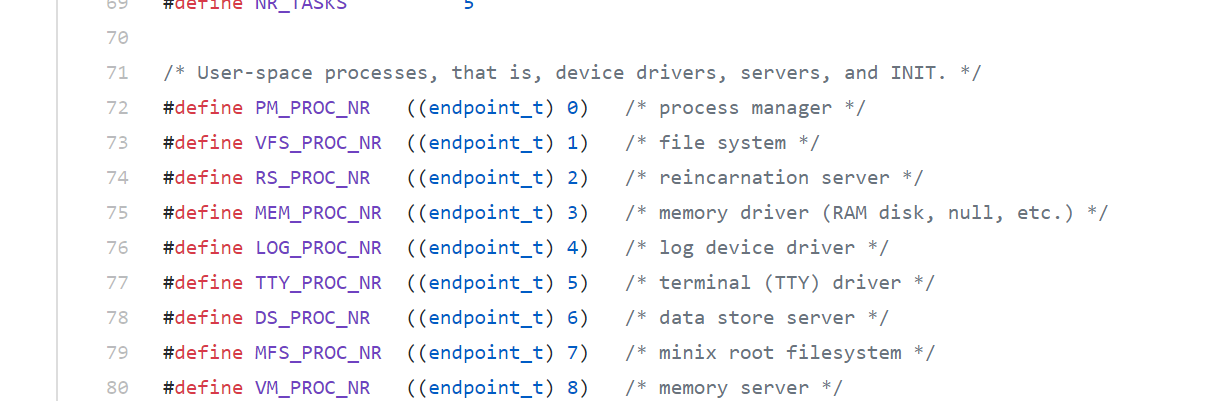
\includegraphics[scale=0.25]{fig/rc5_const}
\end{figure}
Problem of this design:
\begin{itemize}
	\item You need to keep track of the number for collision.
	\item These are handled by preprocessor.
	\item Accessible every where, assigning constants of \texttt{SPADE} to a variable of \texttt{FileType} doesn't make sense. 
\end{itemize}
\end{frame}

\begin{frame}{Critique on enumeration type}
\begin{itemize}
	\item Enumeration type in C++ is tightly connected to integer types. You probably need to constantly change them into integers / from integers. 
	\item Enumeration type lacks NULL/Invalid number. The compiler also doesn't keep track how many discrete value are there. 
	\item The process of reading an enumeration from user input usually involves a large switch. We need to keep retyping the name of the enumeration item. This is no better than a simple \texttt{const}.
	\item They are still accessible everywhere! You can access the enumeration item without specifying the category of the value.
	\item Take a look at C++ 11's newly (not very new after all) introduced \textit{Enumeration Class} for more detail. 
\end{itemize}
\end{frame}

\begin{frame}[fragile]{Buffer, flush and performance}
\textit{Buffering} have a potential problem. If your program crashed at some point, information in the buffer will be lost and thus not print out (for this reason \texttt{cerr} is not buffered). And there is an extra overhead of maintaining the consistence of the C++ style streamed IO with C style \texttt{printf}, \texttt{puts}... 

Why do we need such buffer? The reason is actually performance, flushing the buffer, or printing things onto the screen requires an interaction with the operating system, which is very expensive!

Buffer is an attempt the number of such interaction by trying to send as much text as possible out at once. Compare:

\begin{minted}{c++}
for (int i=0; i<10000; i++) cout << "Hello" << endl;
for (int i=0; i<10000; i++) cout << "Hello" << "\n";
\end{minted}
Generally the first one could be at least 3 times slower than the second one. This will be significant in the runtime of your program since your projects are often IO heavy (outputs a lot).
\end{frame}

\begin{frame}[fragile]{Tips on working with input stream}
\framesubtitle{Avoid parsing whenever possible!}
Specifically, avoid using \texttt{getline()} and \texttt{getch()} whenever possible. The C++ extractors has a very nice property: if you try to extract numbers or strings, the extractor automatically ignores blank characters. This means you only need to focus on the question of 
\begin{center}
	\textit{WHAT is the next thing I need?}
\end{center}

instead of thinking 
\begin{itemize}
	\item WHERE is the next thing I need?
	\item Is what I need on the next line?
	\item Is there a space or a tab before what I need?
	\item How do I get rid of that space / tab / newline?
\end{itemize}
\end{frame}

\begin{frame}[fragile]{Tips on working with input stream}
\framesubtitle{A VG101 Problem}
Recall the following VG101 problem (guess lots of you suffered...):
\begin{figure}
	\centering
	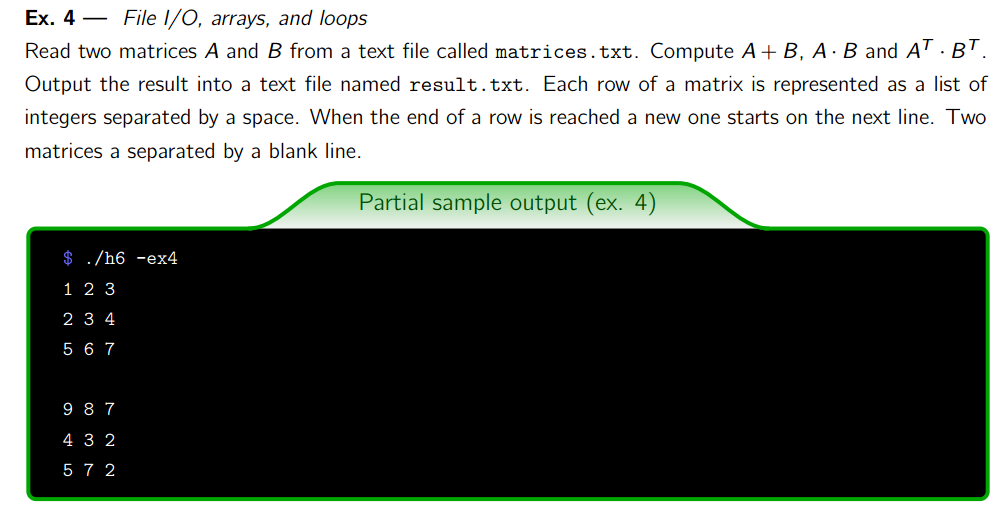
\includegraphics[scale=0.4]{fig/rc5_vg101}
\end{figure}
\end{frame}

\begin{frame}[fragile]{Tips on working with input stream}
\framesubtitle{The failed state}
If you try to extract invalid things from the stream, the stream enters a so called \textit{Failed State}. 

Two typical situation where a input stream will enter a fail state is when you try to extract things from an empty stream (all things in the stream has be extracted). Or you extracted the wrong type.

In general the second situation should be avoided. If you are not sure what next thing is, use a string to accept it. Transform the string into expected type later.

You can test whether a stream is in a valid state (very often if there is still thing remains in the stream) by simply \texttt{if(stream)}.

A very commonly used idiom to extract everything is:

\begin{minted}{c++}
int num; while(cin >> num) /* Do something here */;
\end{minted}

Please note that extractor operator returns an reference of the left hand stream.
\end{frame}

\begin{frame}[fragile]{Tips on working with file streams}
File streams are very much like \texttt{cin} or \texttt{cout}. Please note the difference of \texttt{ifstream} and \texttt{ofstream} and \texttt{fstream}. 

File streams can be opened on construction:
\begin{minted}{c++}
ifstream inputFileStream("input.txt");
\end{minted}
Above code opens \texttt{input.txt} with a \texttt{ifstream}. Please note if the file doesn't exist or failed to open, your \texttt{inputFileStream} will be in a failed state. Remember to check!

Although you can use \texttt{inputFileSteam.close()} to close the stream (and clear its buffer), but you don't actually need to. Remember the stack unwinding example we have before? Standard libraries' file stream are exactly such objects. Its deconstructor will take care of the closing and freeing the file.

\end{frame}

\begin{frame}[fragile]{Use \texttt{istringstream} as parser }
A \texttt{stringstream} can either act be an input stream, or an output stream. They are very different! 

\texttt{istringstream} needs to be ``attached" to a string. This can be down by either passing the string in on construction or use its \texttt{.str()} method. The stringstream, unlike \texttt{cin}, doesn't consume the string, instead it attach a ``pointer" to the string. Ideally:

\begin{minted}{text}
123 abc def Hello world  |  123 abc def Hello world
|<-sstream               |     |<-sstream 
\end{minted}

Right side is after extracting 123 through \texttt{sstream >> intVar;}

\texttt{istringstream} is especially useful in treating data acquired from \texttt{getline}. 

 \alert{If you need to use the same \texttt{istringstream} object for multiple strings, you need to clear it when changing string}. 
\end{frame}

\begin{frame}[fragile]{Use \texttt{ostringstream} as string builder}
From time to time we need to convert different type of data into a string. For example, information about a student is described by:
\begin{minted}{c++}
strcut Student {
    string name; int grade; Date birthday; double GPA;
};
\end{minted}
And you need to turn such stuctures into below format
\begin{minted}{c++}
%name, %grade grade, %YYYY-MM-DD, gpa = %gpa"
\end{minted}
You can setup an \texttt{ostringstream}. You simply push into the stream as if it is \texttt{cout}, finally you call \texttt{ostringstream.str()} to get the result. 
\begin{minted}{c++}
oss << name << "," << grade << " grade" << ... 
\end{minted}
The design of the stream makes it very efficient in dealing with large amount of text. For example you can use it to prepare data to send over the Internet.
\end{frame}

\subsection{Recurse Recursively}
\begin{frame}{Recursion is the art of abstraction}
A typical processes of designing a recursive function goes as follows:
\begin{itemize}
	\item Be very clear first about the abstraction of the function you needed to input.
	\item Specify a base case, a set of input where the answer is immediately known (or can be calculated in a few steps).
	\item Assume that your abstraction actually works for input ``simpler" than the current input (closer to the base case). Use this assumption to build your program.
\end{itemize}
You might find these steps surprisingly similar to a mathematical induction. That's true. They are similar and that's very useful.
\end{frame}

\begin{frame}[fragile]{Recursion is the art of abstraction}
\begin{minted}{c++}
// REQUIRES: list is not empty
// EFFECTS:  returns largest element in the list
int largest(list_t list) {
    int first = list_first(list);
    list_t rest = list_rest(list);
    if (list_isEmpty(rest)) return first;
    return max(first, largest(rest));
}
\end{minted}
\begin{itemize}
	\item The abstraction is specified in the header.
	\item The base base is where list contains just one element.
	\item In the last line, assume abstraction works in simpler case (hope you see why \texttt{rest} is ``simpler" than \texttt{list}). Thus \texttt{largest(rest)} returns the largest of the remaining list.
	\item The largest number can either be the largest of the remaining number, or the first number. 
\end{itemize}
\end{frame}

\begin{frame}[fragile]{Example: Quick sort algorithm}
A quick sort algorithm sorts a array in a quick way (I know that sound like bullshxx!). But list basic steps as following:
\begin{itemize}
	\item Select an element in the array. We simply use the first element. We call this element \texttt{pivot}
	\item We need to \textit{partition} the array. We need to move the elements less than the pivot to the left and elements larger than pivot to the right. Note we assume on the order of the elements left of the pivot (or elements on the right of the pivot).
\begin{minted}{text}
6 5 3 8 -1 7 3 9 11 -4   | 5 3 -1 3 -4 6 8 7 9 11
|<- pivot                |             |<- pivot
\end{minted}
	\item Call \texttt{QuickSort} on the both sides of the pivot.
\end{itemize}
The majority of the work lies in the partition step. 
\end{frame}

\begin{frame}{A usual Quick Sort}
\texttt{$-->$ code/rc5qsort/nonrec.cpp}
\inputminted{c++}{code/rc5qsort/nonrec.cpp}
\end{frame}

\begin{frame}[fragile]{Our Quick Sort}
Suppose we are using our list interface (in the project!). 
\begin{itemize}
	\item Suppose \texttt{QuickSort} is a function that takes in a list and returns a sorted list. Remember this is abstraction. Base case is when the list is empty.
\begin{minted}{c++}
list_t qSort(list_t lst); // Returns sorted lst 
\end{minted}

	\item Our computation goes as follows, we first acquire a the partion-left part and partition-right part. We call \texttt{qSort} on both parts and concatenate left, pivot and right part:
\begin{minted}{c++}
list_t sorted = cat(qSort(left), pivot, qSort(right)) 
\end{minted}
	\item The left part are simply numbers less than pivot, the right part are simply numbers greater than pivot.
\begin{minted}{c++}
list_t left = filterLess(lst, pivot);
list_t right = filterGreater(lst, pivot);
\end{minted}
	\item And we are done. Now we simply copy everything into one place.
\end{itemize}
\end{frame}

\begin{frame}[fragile]{Our Quick Sort}
And here is the famous (almost) one-line quick sort
\begin{minted}{c++}
list_t qSort(list_t lst) {
   if (isEmpty(lst)) return lst;
   int pivot = list_first(lst);
   return concatenate(
       qSort(filterLess(list, pivot)),
       pivot,
       qSort(filterGreater(list, pivot))
   );
}
\end{minted}
Now it just leaves us to implement the filter function and the concatenate function. But these two functions should be very easy. You have implemented the filter function in your project right? 
\end{frame}

\begin{frame}{Why not references and pointers?}
Think about it, why this seems much easier (clearer, hopefully you do feel that way)? 

In the traditional code, all functions works on the same array. We must manually control the process of copying, moving, etc. We are thinking in terms of \textit{operations}, detailed step to be performed.

But the the new code, we can now begin think of data. We stop focusing on the concrete steps, but simply
\begin{center}
	What should I do with the data? \\What is the expected input and the expected output?
\end{center} 
It is the computation we needed to focus. 

This is not easy. The immutability of the data and the fact that all functions are pure allows us to do such thing. Every function does calculation on its own and does not impact the outside world.
\end{frame}

\begin{frame}[fragile]{Bridging the old perspective}
Consider the following problem:

\vspace{0.1in}
\structure{Write a function \texttt{isMoreOdd} that takes a list $(a_0, a_1, a_2, ..., a_n)$ and returns $\Sigma_{i=0}^n i^2a_i$ (we call this an $s$-sum) Assuming the list is non empty.}
\vspace{0.1in}

An example as follows:

\begin{minted}{text}
a_i: 6  5  3  8  -1  7  3 
 i : 0  1  2  3  4   5  6
\end{minted}

We follow our usual steps. The abstraction is self-explanatory. The base case is also easy (a single element list). But the problem lies in the third step. 

It seems that knowing $s$-Sum for for the rest of the list doesn't help on the reducing the problem to a simpler point. 

It would still be most desirable to have some sort of ``accumulator", something that registers a partial sum, a piece of information that ``sums" up the elements before a certain point.
\end{frame}

\begin{frame}[fragile]{Accumulator passing style}
This is still possible. Such construct is so common that gets its own name. We call this \textit{Accumulator passing style} (APS). 

\begin{minted}{c++}
int helper(list_t remain, int index, int acc) {
    if (isEmpty(remain)) return acc;
    acc += index * index * list_first(remain);
    return helper(list_rest(remain), index + 1, acc);
}
list_t strangeSum(list_t list) { 
    return helper(list, 0, 0); 
}
\end{minted}

How does this work? 

The essential idea is to sum up the necessary information into two (could be more) accumulators. We essentially created a sort of running sum.
\end{frame}

\begin{frame}[fragile]{Accumulator passing style}
We then further note the abstraction of the helper function.

The function \texttt{helper} takes the index of the first element in the remainder list and a partial sum of the elements before, and returns the $s$-sum of the entire list.

In this way we transform our original problem of finding out \texttt{helper(list, 0, 0)}. On each recurse call, we extract the first element, and use it to update our accumulators, and passed that on to the next call. 

\begin{minted}{text}
helper([6  5  3  8  -1  7  3], 0, 0)
helper([5  3  8  -1  7  3], 1, 0)
helper([3  8  -1  7  3], 2, 5)
helper([8  -1  7  3], 3, 17)
helper([-1  7  3], 4, 89)
helper([7  3], 5, 73)
helper([3], 6, 248) = helper([], 7, 356) :=356
\end{minted}
\end{frame}

\begin{frame}{Remarks}
\begin{block}{Understand APS in a broad sense}
	APS is extremely useful. In many sense this technique is very similar to loops, which you might feel more comfortable to deal with. On the other hand an accumulator can be more than just an sum of numbers. It could be any information you need to keep track of (for example, if the number before forms an arithmetic sequence, and if they do, what is the increment). 
\end{block}

\begin{block}{Recursion and correctness}
	It's extremely difficult to write correct code! It would be nice if we can formally prove that our code is correct. Since the usual procedural code involves state, this proof can be very complex. 
	
	But if you express the idea using abstraction, proving correctness is very simple and forward. A good recursion construction is almost always correct, and you can prove it! Write once and be free of testing and bug. What a nice thing!
\end{block}
\end{frame}
